\documentclass[DM,lsstdraft,PL]{lsstdoc}

%\renewcommand{\putlogo}{
%  \def\@lbsize{0.75}
%  \begin{center}
%   \resizebox{\@lbsize\textwidth}{!}{\includegraphics[scale=0.04]{lsst_logo}}
%   \end{center}
%}


\begin{document}

\setDocTitle    [DM Risk Process]
                    {\color[rgb]{0.16,0.42,0.57} \sf ~DM Risk
                    Management Process}
\setDocAuthor   {William O'Mullane, Tim Jenness}                % the author(s)
\setDocApprove  {DM project manager}              % approval by ...
\setDocIssue    {01}                        % the issue
\setDocRevision {D}                        % the revision
\setDocRef      {LDM-512-\docIssue} % the reference code
\setDocDate     {\today}              % the date of the issue
\setDocStatus   {Draft}                    % the document status
\setDocCompact  {true}
%\setDocLocalLogo     {}
%
% a short abstract
%
\setDocAbstract {This document defines the risk management process for DM within the overall LSST Risk management process.  Some text in this document has been borrowed from Gaia DPAC, in particular Ron Drimmel worked on this originally. 
}

%
% the title page
%
\mktitle

%
%   Revision history
%
\begin{docHistory}
\addtohist{D}{1}{22-01-2017}{WOM}{Creation}
\end{docHistory}

%
%   TOC
%
\newpage
\setcounter{tocdepth}{3}
\tableofcontents
\newpage

%
% It's all yours from here on
%

\section{Introduction \label{sect:intro}}

Risk management has become a standard element in project management. In simplest terms, all "risk management" means is anticipating problems and taking actions to avoid these problems: good practice for any complex endeavour. Formalising a risk management plan insures that risk management becomes a standard and regularised task in running a project.

\subsection{Scope \label{sect:scope}}

This document defines the risk management process for the Data Management (DM) part of the LSST project.

\subsection{Applicable Documents \label{sect:appdocs}}
\begin{tabular}[htb]{l l}
\citell{LPM-20} & Risk \& Opportunity Management Plan\\
\end{tabular}

\subsection{Reference Documents\label{sect:references}}

\renewcommand{\refname}{}
\bibliographystyle{gaia_aa}
\bibliography{lsst,gaia_livelink_valid,refs,books,refs_ads}

\newpage
\subsection{Acronyms}
The following table has been generated from the on-line Gaia acronym list:
\newline\newline%decrement table counter so table sin doc start at 1.
\addtocounter{table}{-1}
\begin{longtable}{|l|p{0.8\textwidth}|}\hline
\textbf{Acronym} & \textbf{Description}  \\\hline
CU&Coordination Unit (in DPAC) \\\hline
DM&Data Management \\\hline
DMLT&DM Leadership Team \\\hline
DPAC&Data Processing and Analysis Consortium \\\hline
DPACE&Data Processing and Analysis Consortium Executive \\\hline
DPC&Data Processing Centre \\\hline
ECSS&European Cooperation for Space Standardisation \\\hline
JIRA&issue tracking product (not an acronym, but a truncation of Gojira, the Japanese name for Godzilla) \\\hline
LSST&Large-aperture Synoptic Survey Telescope \\\hline
OR&Observation Report \\\hline
PC&(DPAC) Project Coordinator \\\hline
RMT&Risk Management Team \\\hline
TCAM&Technical Control/Account Manager \\\hline
TCT&Technical Control Team \\\hline
\end{longtable}
 % generated by the acronyms.csh (GaiaTools)

%%%%%%%%%%%%%%%%%%%%%%%%%%%%%%%%%%%%%%%%%%%%%%%%%%%%%%%%%%%%%
\newpage

\section{Project Summary \label{sect:project}}

%-Objectives of LSS. reference to Project overview .\\
The goal of the Large Synoptic Survey Telescope (LSST) project is to conduct a 10-year survey of the sky that will deliver a 200 petabyte set of images and data products that will build a large-aperture, wide-field, optical imaging facility designed to address some of the most pressing questions about the structure and evolution of the universe and the objects in it.  For more details see \citellp{Document-15077}

The DM (Data Management) subsystem represents the science ground segment of the LSST, responsible for the data processing of the data stream. Its objective is the production of a set of science pipelines to produce the LSST Science Products \citellp{LSE-163}. 

For further details of the responsibilities within DM see the Management Plan\footnote{Update due April 2017} \citellp{LDM-294}.


\newpage

\section{Risk management principles \label{sect:principles}}

Risk management process in DM:
\begin{itemize}
\item Derives naturally from \citell{LPM-20} just extending the process to all parts of DM.
\item Should initially be simple and straight-forward: The risk management plan can evolve as needed.
\item Should be independent of any tool adopted to assist in risk management.
\item Should be a supporting activity to the project and not a burden: Administrative overhead should therefore be kept to a minimum.
\item Should periodically reassess risks, to take into account experience, evolution of the project, changing context of project, etc.
\item Should take place at the DM level first with major risks promoted to LSST level.
\end{itemize}


\section{Risk definition \label{sect:definition}}
%\section{Risk management approach \label{sect:approach}}

\subsection{Domains of risk}
See also the definitions section of \citeds{LPM-20}.

In the general context of project management, a risk is defined as a threat to project success because it has a negative impact on cost, schedule or technical performance.

As the primary products of DM are scientific in nature, any threat that could reduce or limit the scientific performance of the data processing can be considered as a risk. This includes factors that may have a  negative impact on the precision of the data processing results. It is worth noting in this context that computing performance of the implemented SW systems can have an indirect impact on scientific performance, as implemented SW must be able to process a certain volume of data in a limited amount of time. Assuming that SW has been efficiently implemented, this constraint can place limits on the algorithms that can be adopted; if the computational cost of an algorithm is too large a less accurate (but faster) algorithm would be preferred. Therefore, if something might increase the computational cost of the data processing (i.e. an increase in the number of objects to be processed, or an increase in algorithmic complexity to reach a desired scientific precision, etc.), it represents a risk to the scientific performance.

\subsection{Risk validity/Identification}

A valid DM risk impacts one or more of the three domains: resources, schedule or performance (see previous section).

One of the first tasks of the risk management process is to consider and discuss proposed risks, determine their validity and select those risks which are to be documented (see task one in section \ref{sect:strategy}).

Here are some examples of proposed risks  and the outcome expected from such a discussion.

\subsubsection*{Proposed risk 1:}

Real data is far more complex and quite different to the simulated data. Processing especially Alerts production is more computationally intensive and complex.
Practically all missions experience this.

Expected conclusion:\\
Not accepted to be recorded as a risk because the proposal itself points out that real data will be more complex, so it is normal work to design, develop and plan for it.

\subsubsection*{Proposed risk 2:}

Calculations made by  one group indicate that the hardware for the computationally intensive tasks it needs to perform does not scale well. Delay may occur while the technical solution is investigated.

Expected conclusion:\\
This risk could be easily recorded with related severity and likelihood criteria. The initial actions and mitigation processes would be put into place,  for example: \\
a)	look for alternative hardware solutions (may increase cost, but could recover schedule)\\
b)	set a firm date for the first technical assessment and call a DMLT meeting to address alternative and solutions.

The first example above is intended to illustrate a poor or bad risk proposal and the second is an example of a likely and reasonable proposal.

In general, a properly identified risk is composed of both cause and consequence, \citeds{LPM-20} identifies the following list of assessment criteria:
\begin{enumerate}
\item \textbf{Identification : }
identifying elements of risk or opportunity in the subsystem or Project.
\item \textbf{Establishing  time  frame :}
    determining  the  likely  time at  which a  risk or  opportunity event would come to pass.
\item \textbf{Assessing  probability :  }
  estimating  the  probability  that  an  undesirable (for  risks)  or desirable (for opportunities) event may occur.
\item \textbf{Assessing  severity :}
   gauging  the  severity  of  the  impact  that  such  an  event  would  have on the status of the project if the event were to occur.
\item \textbf{Developing risk /opportunity handling options :}
\begin{itemize}
\item  For  risks: developing  plans to  avoid, accept, mitigate, or transfer
\item  For opportunities: developing plans to permit or promote
\end{itemize}

\item \textbf{Developing  a  management  response : }
 consider  how  the  project  may  respond  if  the event should occur
\end{enumerate}

In addition for DM we should determine if the risk merits promotion to the project level risk register.

\subsection{Risk scoring: severity and likelihood \label{sect:scoring}}

Risk scoring is an attempt to qualitatively assess risks, and thus serves as an aid to objectively decide whether a risk merits attention, i.e. whether preemptive action should be taken to address the risk. Typically the two most important qualities of a risk that determines its seriousness is \emph{severity} and \emph{likelihood}.

For DM risk management, we adopt the severity and likelihood scales detailed below.

Risk severity is an evaluation of the consequences should a risk occur, and is measured using the following scale:
{\color{red} Not exactly what happens in LSST .. we may need to look at this}

\begin{tabular}{|l|l|p{0.75\linewidth}|} \hline
Score & Severity & Consequences of occurrence \\ \hline
5 & Catastrophic & Impact on resources, schedule and/or performance leads to the termination of the project. \\ \hline
4 & Critical & Final data production is compromised, either by significantly degrading its final quality so that several mission requirements will not be met,
and/or delaying its release by more than a year. Delay in first light  is required. Major resource re-allocation or acquisition perhaps at the telescope. \\ \hline
3 & Major & Occurrence causes a delay in the delivery of a non schedule critical component of more than one cycle, impacting the schedule of more than one part of DM over more than one cycle. Resources must be re-allocated between group or additional funds required, requiring intervention of LSST Project Manager. Final products are potentially compromised, so that one or more requirements will not be met unless new methods are developed or new resources can be found. \\ \hline
2 & Significant & Occurrence implies the delivery of a low quality product (component/algorithm/data is sub-optimal, not up to specs, incomplete, etc.) on time, or a delay is necessary to reach spec. Re-assignment of resources are necessary, but adjustments can be made within the group. Schedule of more than one part of DM is compromised, but original schedule can be re-attained after 1 cycle (some development cycle milestones must be postponed to next cycle, but no more). Final products may be compromised, but all mission requirements are met. \\ \hline
1 & Negligible & Occurrence implies some slight degradation in the quality of delivered product. Schedule of current cycle stressed, even compromised, but no impact on subsequent cycles. \\ \hline
\end{tabular}

Note: If any one of the consequences of a given severity applies, then the risk is at that specified severity level.
Also note: Severity is determined according to consequences to the DM as a whole.

Risk likelihood is an estimate of how likely the risk may actually happen. \figref{fig:lh} shows the scale from \citeds{LPM-20}

\begin{figure}
\begin{center}
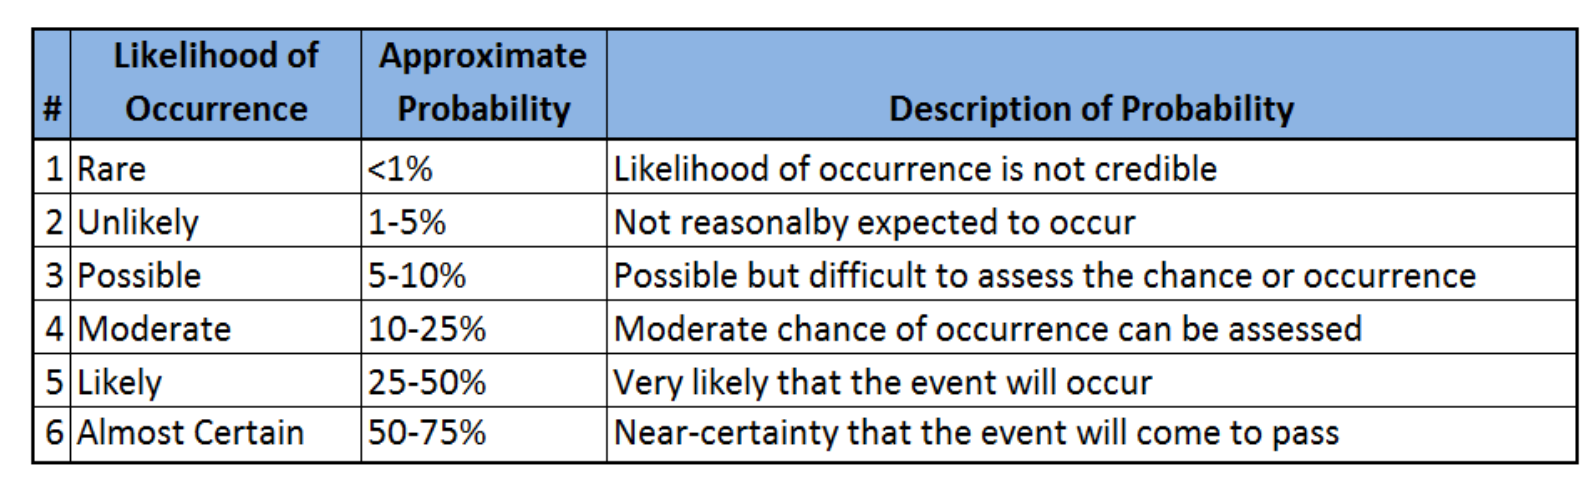
\includegraphics[width=0.8\textwidth]{images/lh}
\caption{Likelihood scale for risks from \citeds{LPM-20}.\label{fig:lh}}
\end{center}

\end{figure}

These two scales (for severity and likelihood) define a two-dimensional space on which a given risk may be quantitatively mapped and thus assessed. A single code that describes the risk assessment can be constructed from these two scales, for example an A1 risk is a risk with minimum likelihood and minimum severity, while an E2 risk is a risk with significant impact that will certainly happen at least once in the next development cycles.

An acceptance regime (used to decide whether to accept a risk or take action to reduce the risk) is defined in the severity-likelihood plane in the next section \ref{sect:acceptance}.

It may be useful to reduce the two measures above to a single \emph{risk index}, for the purpose of prioritising a list of risks or monitoring risks over time. An example of a risk index is shown in figure \ref{fig:riskindex}, showing a rating going from "Very Low" to "Very High".

  \begin{figure}[H]
  \begin{center}
  	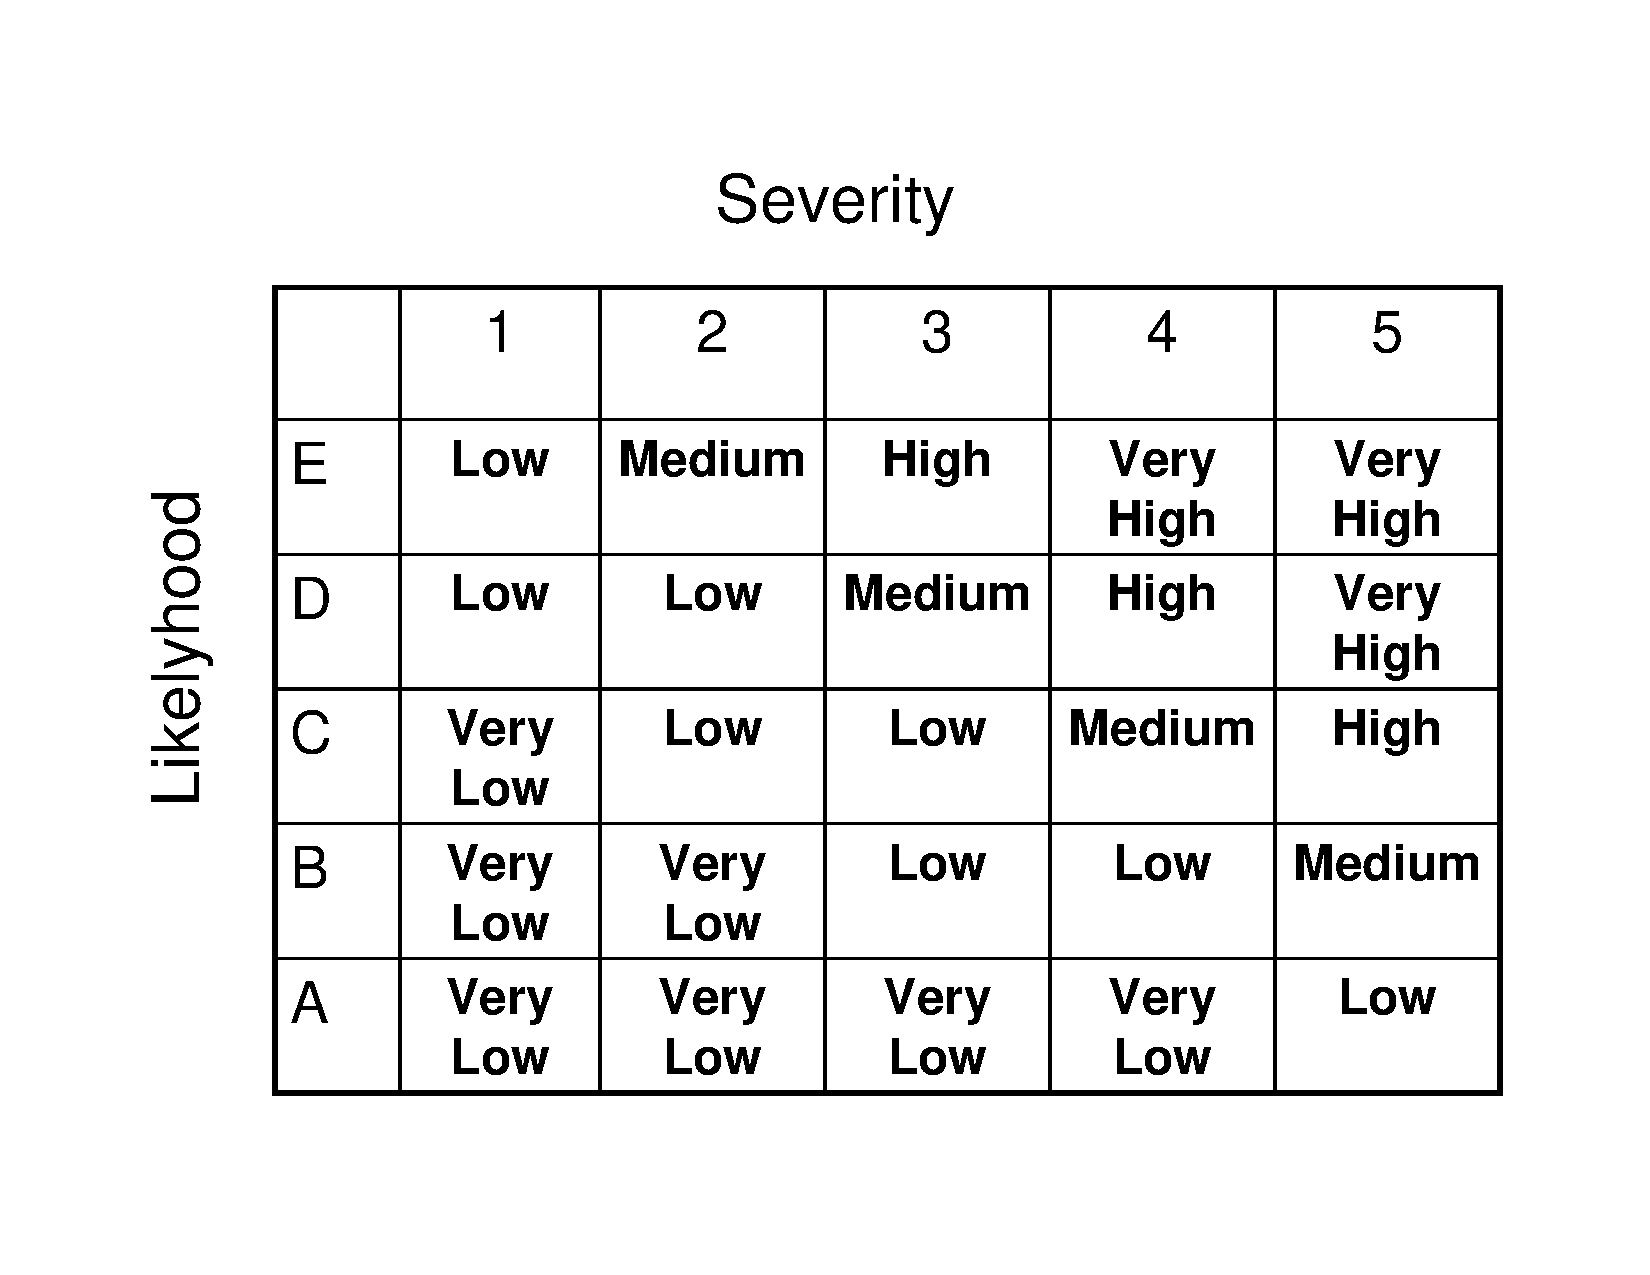
\includegraphics[scale=0.5]{images/RiskIndex}
  \end{center}
\vspace{-2cm}
\caption{Risk Index \label{fig:riskindex}}
   \end{figure}

Finally, it is worth mentioning that while the above scores and indices are quantitative they are still subjective measures, and thus can only serve as aids in the risk management process. There is no substitutes for good judgement based on experience.

\subsection{Risk acceptance \label{sect:acceptance}}

The risk scores are used to define criteria for acceptance or an acceptance regime in the severity-likelihood plane. This acceptance regime is shown in figure \ref{fig:regime}.

  \begin{figure}[H]
  \begin{center}
  	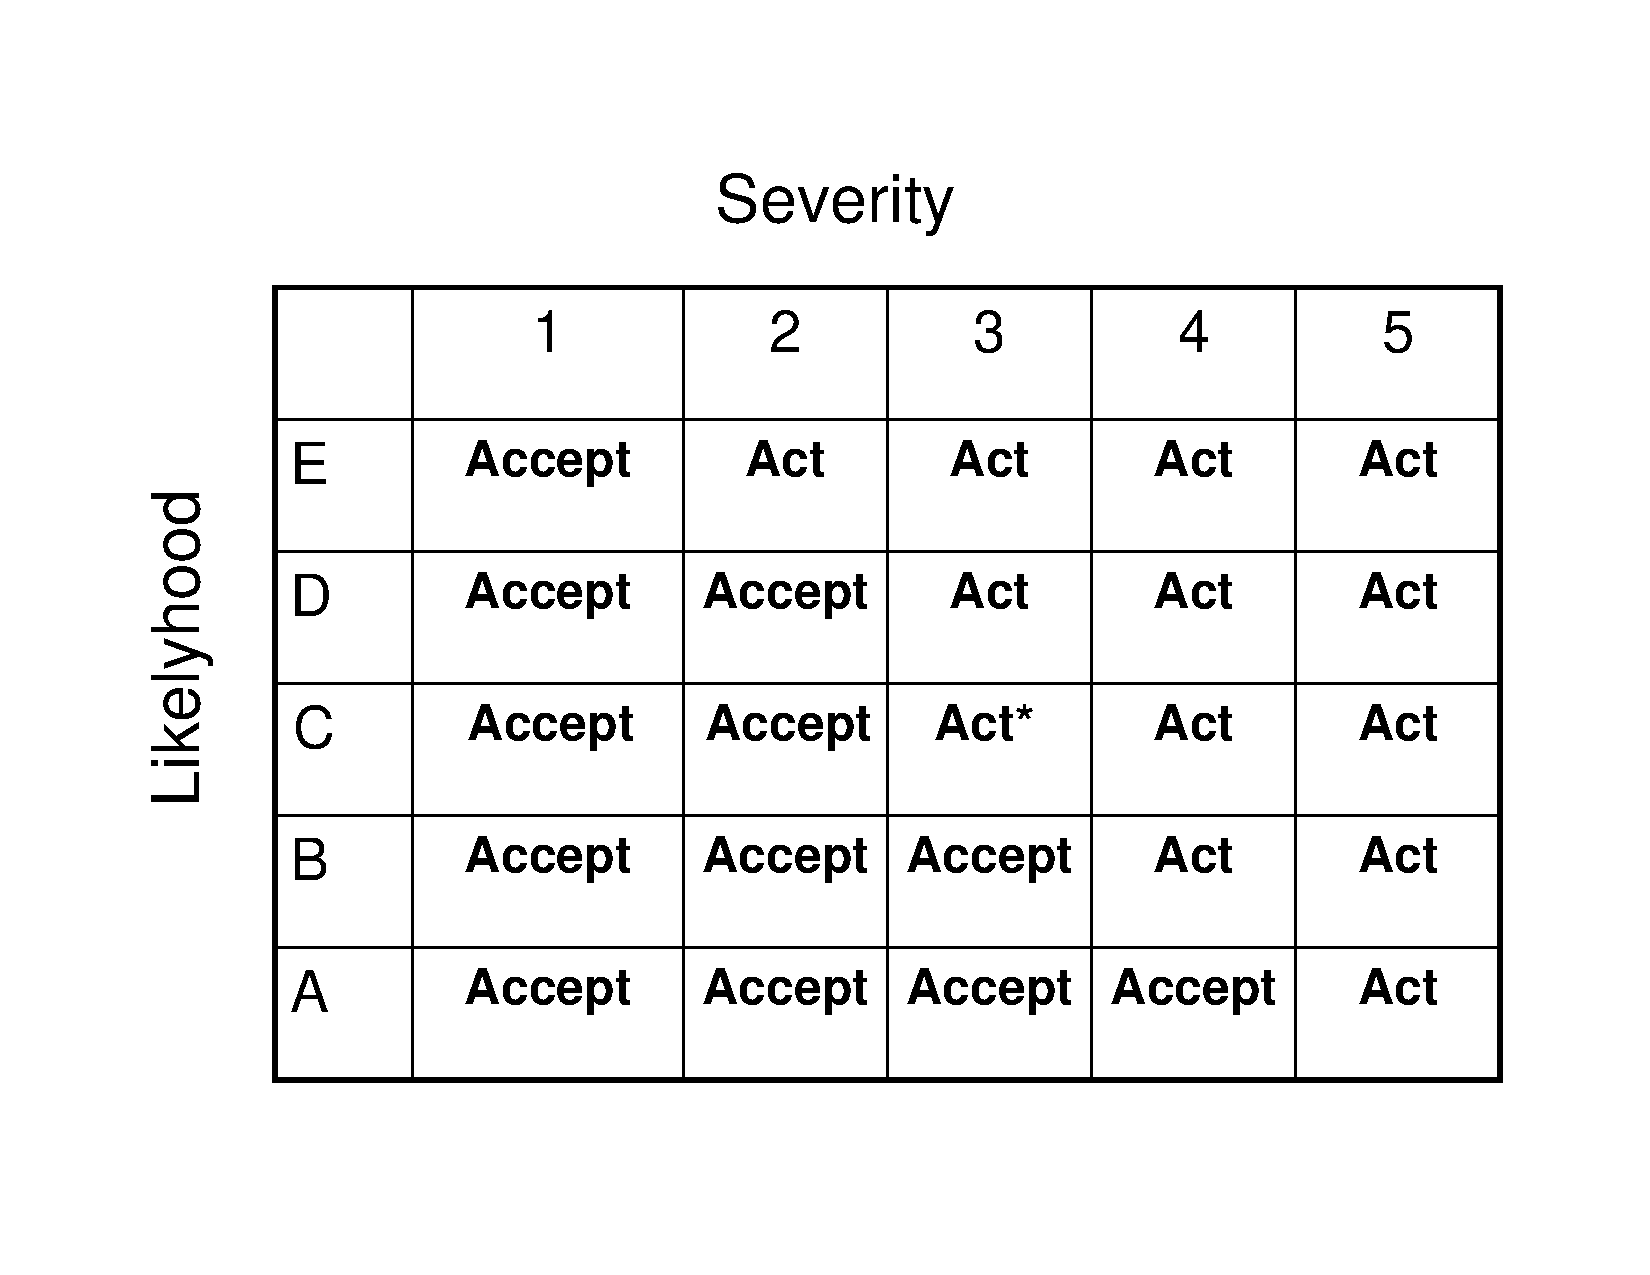
\includegraphics[scale=0.5]{images/AcceptanceRegime}
  \end{center}
\vspace{-2cm}
\caption{Acceptance regime \label{fig:regime}}
   \end{figure}

It should be noted that it is not required for a risk to fall in the acceptance regime for the RMT to recommend acceptance, particularly risks with a 'C' likelihood and a '3' severity criteria (see task 5 in section \ref{sect:strategy}).


\section{Risk/Opportunity  management process \label{sect:strategy} }

\subsection{Roles and responsibilities  \label{sect:org} }

\subsubsection{LSST members}
The approach in DM is  that all LSST  members are free to identify risks through the DM risk management project in Jira.


\subsubsection{Risk Management Team}

The RMT is composed of the following: the DM Project Manager, the DM System Engineer and the DM Quality Assurance Manager{\color{red}Do we have such a role?}  . This list can be extended to some technical experts depending on the risk nature.

The RMT shall be led by the PC and be responsible for:
\begin{itemize}
\item Maintaining the DM risks in the LSST Register.
\item Any reissues of this document.
\item Issuing a DM Risk Report after each risk management meeting.
\item Completing a risk management cycle, as described in section \ref{sect:strategy}, at least once per development cycle.
\item Acknowledging new risks and monitoring registered risks, as specified in section \ref{sect:tasks}.
\item Recommends an assessment that the DMLT approves or modifies.
\end{itemize}
Risk management meetings are held by the risk management team (RMT) at least twice per year, and at least one month prior to regularly scheduled DMLT meetings. The risks actions may be  monitored monthly during the DMLT teleconference.

\subsubsection{DMLT}

It is the DMLT{\color{red} OR TCT ?} that has the authority to:
\begin{itemize}
\item Assess the acknowledged risk or, if any, approve the RMT risk assessment.
\item Decide on actions to mitigate risks as needed, approving proposed action from the RMT or formulating new actions.
\end{itemize}

\subsubsection{Local Risk Manager}
Each DM group shall designate a Local  Risk Manager (which could be the TCAM but need not be). This person shall be responsible for:

\begin{itemize}
\item Identifying and submitting in JIRA any new risks that will be reviewed by the RMT.
\item Validating the recommendations of the RMT on existing risks affecting the group.
\item Communicating to the RMT any action carried out to reduce identified risks, as well as their effectiveness.
\item When appropriate, or on request of the RMT, indicate for risk, a technical expert in the group that the RMT may contact directly for necessary clarifications.
\end{itemize}

In short, the Local Risk Manager is the contact point for the RMT, and guarantees that there is at least one person in the group management structure to communicate and track the CU risks.

\subsection{Risk management tasks \label{sect:tasks} }

To assure that mitigating actions are completed on a timely basis, risk management will take place on a cyclic basis.

Figure below defines the tasks and responsible that take place over a risk management cycle.
These tasks are based on the ECSS standards (ECSS-M-ST-80C) tailored to the DPAC and proposed here for LSST DM.
Risk management meetings will be held on a regular basis to address these tasks, thus there is one risk management meeting per risk management cycle.

\begin{figure}[H]
\begin{center}
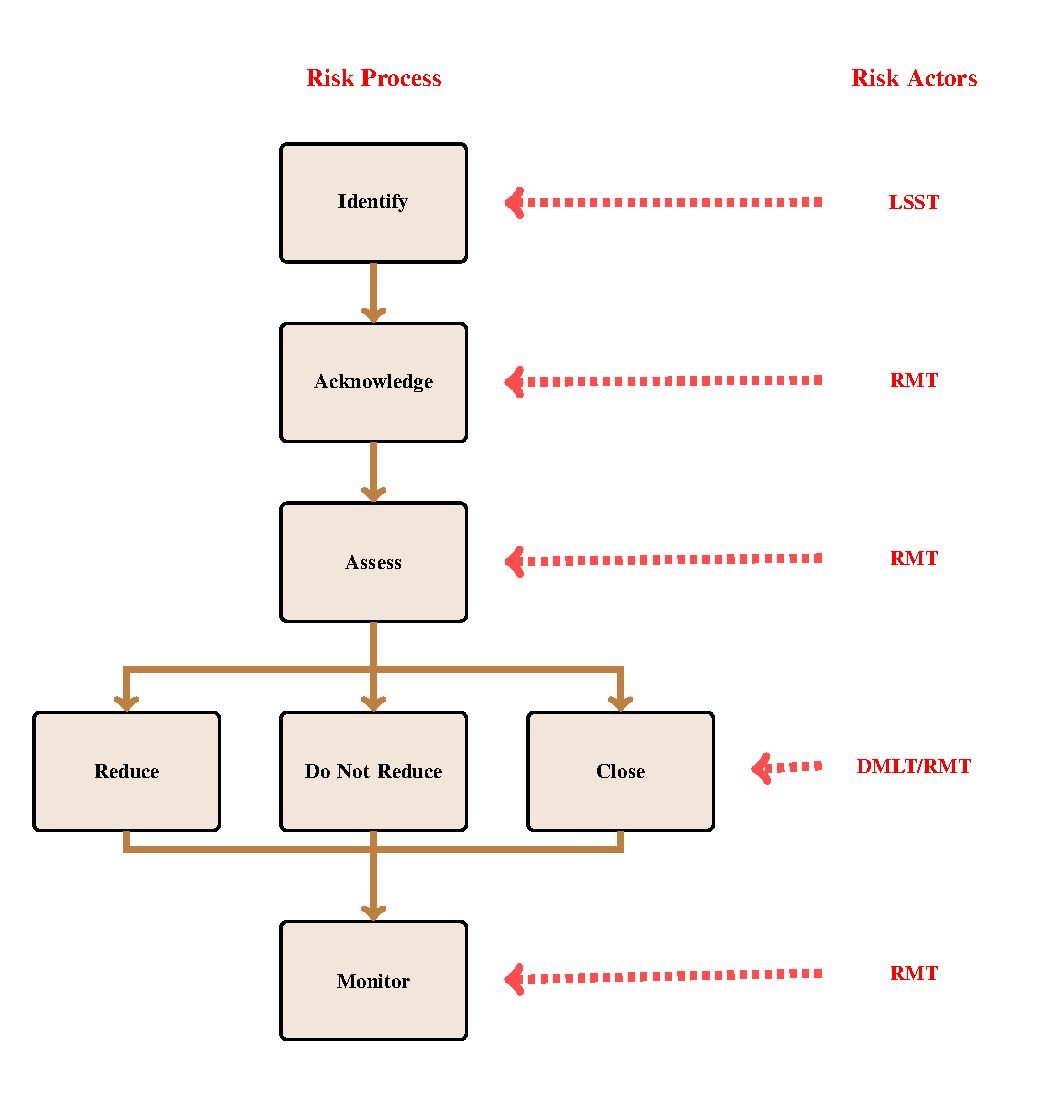
\includegraphics[width=0.8\textwidth]{images/RiskProcess}
\end{center}
\caption{Risk Management Process}
\label{fig:riskprocess}
\end{figure}

\subsubsection*{Task 1: Identify risk scenarios}

It is expected that potential risks will be submitted by various parties in LSST, and indeed input of possible risks should be communicated by the CUs and DPCs.

\subsubsection*{Task 2: Acknowledge the risks}
Any new risks should be reviewed by the risk management team during the risk management meeting to determine their validity. If a new risk is not considered valid, it is closed. The closed risks will be presented to DMLT.
In addition, more general risk scenarios should be contemplated during the risk management meeting to identify any new risks.

\subsubsection*{Task 3: Assess the risks}

For each valid risk, and for all previously identified risks, (re)assess their likelihood and severity, using the scales defined in section \ref{sect:scoring}. The RMT recommends an assessment that the DMLT approves or modifies.

\subsubsection*{Task 4: Reduce the risks}

For those risks that are deemed as "unacceptable", the risk management team will try to define possible actions to reduce risks in terms of occurrence and/or likelihood.
The risk management team needs to balance increasing expenditure to tackle a risk.

All risks ranked as "unacceptable" should have at least one dedicated action.
The RMT should recommend mitigating actions if possible; the DMLT decides on the final actions to be taken, approving the recommendations of the RMT or formulating new actions.

\subsubsection*{Task 5: Do not reduce the risks (acceptance)}

Whether or not mitigation actions are identified, there should come a time in the project when a risk can not be reduced any further. In this case the risk management team should recommend to {\em accept} the risk, even if it does not pass the acceptance criteria defined under task 3.

Risks should also be accepted if the cost to mitigate is greater than the cost of the consequences, obviously. More generally a risk might be accepted if the severity/likelihood of the consequences does not merit the cost to mitigate.

All accepted risks should be re-assessed at the next risk management cycle.

A risk may be closed if it is deemed unnecessary to continue monitoring the risk. This might be because it no longer applies to the project (is no longer a valid risk), or is no longer a significant risk (likelihood is null or no negative consequences). The risk management meeting may identify risks to be recommended for closing.

\subsubsection*{Task 6: Monitor the risks}

After approval, the RMT is in charge of updating and issuing a new version of the Risk register. Feedback from the concerned parties is also necessary so that the risk management team can properly monitor risks. Were recommended actions taken? What were the results? Were risks recommended for acceptance approved or not?

\subsection{Risk management technical implementation \label{sect:technical} }
JIRA has been chosen as our Risk Management Tool in DM, this section describes the technical part of a risk registration and monitoring.


\subsubsection{Use of JIRA as a risk management tool}

{\color{red} Tim -- this is a section for you to update}


JIRA is an issue tracking tool that has been adopted by LSST to assist and coordinate a software development effort distributed throughout the US and Europe. This section describes how JIRA will be used as a risk management tool.

In particular, for a risk reported as a JIRA issue:
\begin{itemize}
\item The automatically generated JIRA issue number will be used as a unique alphanumeric risk identifier.
\item The JIRA Summary serves as the short descriptive title of the risk.
\item The JIRA Description serves as the full description of the risk.
\item Under the JIRA DM Risk Register project, additional customised fields to enter the risk likelihood, and severity. Changes to these fields are automatically logged by JIRA.
\item Recommendations by the RMT are reported in the custom fields "Recommendations" and "Actions".
\end{itemize}


\subsubsection{Risk submission in JIRA}

 When submitting a new risk in JIRA a set of fields are to be fulfilled, some are optional.
{\color{red} THIS NEEDS REVIEW}
 The table below present these fields:
\begin{longtable}{|l|p{0.6\textwidth}|}\hline
\textbf{JIRA field} & \textbf{Description} \\ \hline
Summary    & Summary of the risk  \\ \hline
Description    & Complete description:
\begin{itemize}
  \item Detail of the risk.
  \item Cause.
  \item Possible action.
\end{itemize}
\\
\hline
Consequence  & Description of the consequences in terms of time, resource, performance.\\
\hline
Risk severity (optional)   & See \ref{sect:scoring}. \\
\hline
Risk likelihood (optional)   & See \ref{sect:scoring}. \\
\hline
\end{longtable}

Note that any new risk with a vague description will be \textbf{closed} by the RMT.
After review by the RMT, each registered risk shall have at the following fixed properties :

\begin{itemize}
\item A unique alphanumerical identifier that, once assigned, will not change.  It is solely the task of the RMT to assign this identifier.
\item A short descriptive title.
\item A full description (including both cause and proposed solution).
\item Consequence of the risk in terms of time, resource, performance.
\item The name of the original submitter.
\item The date of submission.
\item Estimated date of occurrence
\end{itemize}

In addition, each registered risk shall have the following transient properties (i.e. properties that change with time) also assigned by the RMT:
\begin{itemize}
\item A severity and likelihood rating, and the derived the risk index.
\item The date of assessment (first assessment coincides with the date of risk registration).
\item Recommended response at time of assessment (reduction or acceptance).
\item JIRA status: assigned, resolved or closed.
\item Actions taken (if any), when and by whom.
\item \ldots
\end{itemize}

The submitter may provide an initial risk rating; in this case these ratings must be re-evaluated by the RMT at time of registration.

The risk identifier may contain information of the source of submission (for example, a CU number), but \textbf{not} the risk assessment scores, as these will change with time.

The list of registered risks at the DPACE level constitutes the DPAC Risk Register. The DPAC Risk Register shall be reissued after each risk management meeting.

\subsubsection{Risk Process Vs JIRA Status \label{sect:JIRA}}


The figure below presents the different JIRA status through the Risk Process, the blue boxes are the JIRA status:

\begin{figure}[H]
\begin{center}
%\includegraphics[scale=0.9]{RiskJIRAStatus}
\end{center}
\caption{JIRA Status through Risk Process}
\label{fig:riskJIRA}
\end{figure}


Note that all 'unacceptable' risk with an 'assigned' JIRA Status have at least one dedicated action monitored in JIRA.

\subsubsection{Risk change tracking}

An identified risk has a natural "life-cycle": a beginning, a middle and an end. These three parts correspond to risk registration, a monitoring phase and eventual risk closing. All risks surviving to the end of project are of course retired at project's end. During its lifespan a risk is constantly monitored and reassessed, perhaps acted on and (perhaps) reduced. In short, a risk accumulates a history.

The history of a risk is essentially a history of all past values of its transient properties. Tracking the history of risks is an important part of risk monitoring.

In addition to the Risk Register, the RMT shall issue a Risk Report from JIRA after each risk management meeting, with summary statistics of the current risks and overall risk trends.


\end{document}
